\chapter{Divisas (FX)}\label{cap:fx}

\section{Convenciones}
Un par \texttt{BASE/COTIZADA} indica cuántas unidades de la cotizada vale una de la base:
EURUSD $=1{,}0850$ significa 1~EUR $=1{,}0850$~USD. Comprar el par es comprar la base y vender la
cotizada. Mayores: EURUSD, USDJPY, GBPUSD, USDCHF, AUDUSD, USDCAD, NZDUSD; el resto son cruces.

\begin{itemize}
\item \textbf{Pip}: 0,0001 (0,01 si la cotizada es JPY) — \py{fx.pip\_size}.
\item \textbf{Lote estándar}: 100\,000 unidades de la base (mini 10\,000, micro 1000).
\item \textbf{Valor del pip} por lote: $0{,}0001\times100\,000=10$ unidades de la cotizada; se convierte
  a la divisa de la cuenta (\py{fx.pip\_value}). En EURUSD con cuenta en USD vale 10~\$; en USDJPY a
  150, $1000/150=6{,}67$~\$.
\end{itemize}

\begin{lstlisting}
python scripts/tamano_posicion.py fx --capital 20000 --riesgo 1 --par EURUSD --tipo 1.0850 --stop-pips 25
\end{lstlisting}

\paragraph{Tipos cruzados.} EURJPY $=$ EURUSD $\times$ USDJPY; EURGBP $=$ EURUSD $/$ GBPUSD. En general,
pasando por USD (\py{fx.cross\_rate}). Si el cruce cotizado se desvía del implícito más que los
spreads, hay arbitraje triangular (\py{fx.triangular\_arbitrage}); en la práctica solo lo capturan los
creadores de mercado más rápidos.

\section{Forwards y paridad cubierta de intereses}
No arbitraje entre invertir en cotizada o cambiar, invertir en base y cerrar con un forward:
\begin{equation}\label{eq:cip}
F = S\,\frac{1+r_{\text{cot}}\,T}{1+r_{\text{base}}\,T}\quad(\text{convención monetaria, } T=\text{días}/360).
\end{equation}
Los \textbf{puntos forward} son $(F-S)/\text{pip}$ (\py{fx.forward\_rate}, \py{fx.forward\_points}). La
divisa con tipo de interés más alto cotiza con \emph{descuento} a plazo.

\section{Carry trade}
Comprar la divisa de tipo alto financiándose en la de tipo bajo cobra el diferencial de tipos:
\begin{equation}
\text{rent.} = \frac{(1+r_b T)S_1 - (1+r_q T)S_0}{S_0} \approx \frac{S_1}{S_0}-1 + (r_b-r_q)T
\end{equation}
(\py{fx.carry\_return}). La paridad \emph{no cubierta} diría que la divisa de tipo alto se deprecia lo
justo para anular el carry; empíricamente no lo hace en promedio (\emph{forward premium puzzle}), y por
eso el carry ha sido rentable\ldots{} con \textbf{asimetría negativa}: sube por la escalera y baja por
el ascensor (1998, 2008, agosto de 2024 con el yen).
\begin{figure}[h]\centering
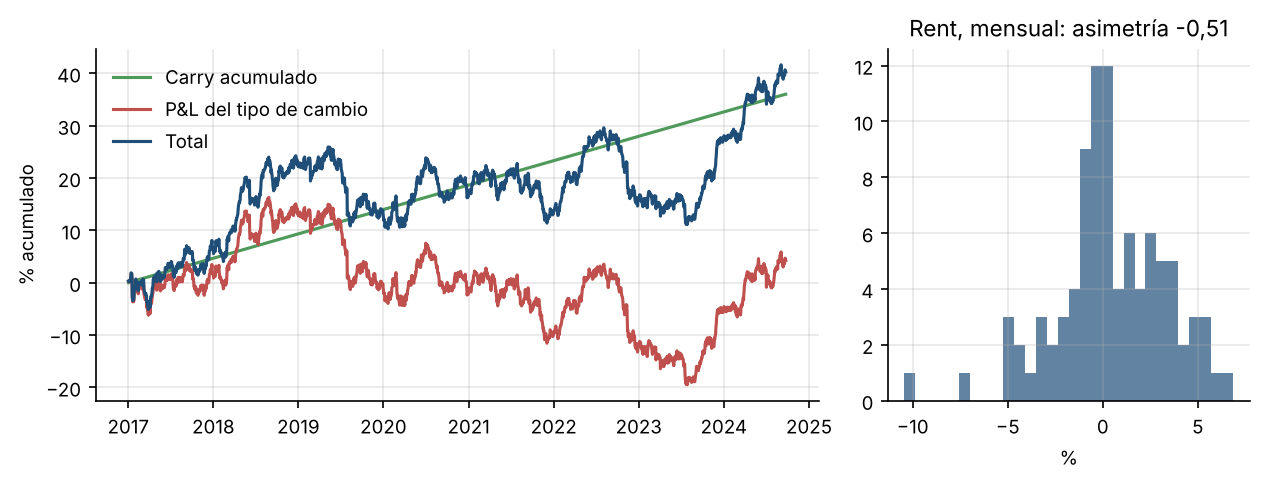
\includegraphics[width=\textwidth]{f08_carry}
\caption{Carry trade simulado: el diferencial se acumula de forma estable, pero el tipo de cambio sufre
caídas bruscas que generan una distribución mensual con cola izquierda.}
\end{figure}

\section{Qué mueve las divisas}
\begin{itemize}
\item \textbf{Diferenciales de tipos reales y expectativas de bancos centrales}: el factor dominante a
  medio plazo. Sigue los tipos a 2 años de cada país y el calendario de reuniones (Fed, BCE, BoJ, BoE).
\item \textbf{Datos macro}: empleo (NFP), IPC, PMI, PIB. El movimiento depende de la sorpresa frente al consenso.
\item \textbf{Aversión al riesgo}: USD, JPY y CHF suelen apreciarse en crisis; AUD, NZD y emergentes depreciarse.
\item \textbf{Términos de intercambio}: CAD y NOK con el petróleo, AUD con el mineral de hierro y China.
\item \textbf{Valor a largo plazo}: la paridad de poder adquisitivo relativa
  $S_{\text{justo}} = S_0\,\frac{P_{q,t}/P_{q,0}}{P_{b,t}/P_{b,0}}$ (\py{fx.relative\_ppp}) es un ancla débil a varios años.
\item \textbf{Flujos e intervenciones}: fixing de fin de mes, repatriaciones, intervenciones (BoJ, SNB).
\end{itemize}

\begin{practica}
En FX el tamaño se piensa en pips de stop y en lotes. Calcula siempre el valor del pip en la divisa de
tu cuenta y vigila la \textbf{correlación} entre pares: largo EURUSD y largo GBPUSD es,
principalmente, una sola apuesta corta en dólares. Ten en cuenta el \emph{swap} nocturno (el carry) que
cobra o paga tu broker y los spreads amplios en la apertura de Sídney y en noticias.
\end{practica}

\begin{ejercicios}
\begin{enumerate}
\item EURUSD $=1{,}0850$, tipo USD 4,5~\%, tipo EUR 2,25~\%. Calcula el forward a 90 días y los puntos
  (\py{python scripts/calculadoras.py forward ...}).
\item Valor del pip de EURGBP para una cuenta en USD con GBPUSD $=1{,}27$.
\item ¿Por qué un carry trade financiado en yenes sufre cuando sube la volatilidad global?
\end{enumerate}
\end{ejercicios}
